
\section{Strike-Slip Benchmark}
\label{sec:benchmarks:strikeslip}

This benchmark problem computes the viscoelastic (Maxwell) relaxation
of stresses from a single, finite, strike-slip earthquake in 3D without
gravity.  Dirichlet boundary conditions equal to the analytical elastic
solution are imposed on the sides of a cube with sides of length 24
km. Anti-plane strain boundary conditions are imposed at y = 0, so
the solution is equivalent to that for a domain with a 48 km length
in the y direction. We can use the analytical solution of \cite{Okada:1992}
both to apply the boundary conditions and to compare against the numerically-computed
elastic solution.

\subsection{Problem Description}

Figure \vref{fig:benchmark:strikeslip:geometry} shows the geometry
of the strike-slip fault (red surface) embedded in the cube consisting
of an elastic material (yellow block) over a Maxwell viscoelastic
material (blue block). 
\begin{description}
\item [Domain] The domain spans the region
\begin{gather*}
0\leq x\leq24\ km,\\
0\leq y\leq24\ km,\\
-24\ km\leq z\leq0.
\end{gather*}
The top (elastic) layer occupies the region $-12\ km\ \leq z\leq0$
and the bottom (viscoelastic) layer occupies the region $-24\ km\ \leq z\leq-12\ km$.
\item [Material~properties] The material is a Poisson solid with a shear
modulus of 30 GPa. The domain is modeled using an elastic isotropic
material for the top layer and a Maxwell viscoelastic material for
the bottom layer. The bottom layer has a viscosity of 1.0e+18 Pa-s.
\item [Fault] The fault is a vertical, right-lateral strike-slip fault.
The strike is parallel to the y-direction at the center of the model:
\begin{gather*}
x=12\ km,\\
0\leq y\leq16\ km,\\
-16\ km\leq z\leq0.
\end{gather*}
Uniform slip of 1 m is applied over the region $0\leq y\leq12\ km$
and $-12\ km\leq z\leq0$ with a linear taper to 0 at y = 16 km and
z = -16 km. The tapered region is the light red portion of the fault
surface in Figure \vref{fig:benchmark:strikeslip:geometry}. In the
region where the two tapers overlap, each slip value is the minimum
of the two tapers (so that the taper remains linear).
\item [Boundary~conditions] Bottom and side displacements are set to
the elastic analytical solution, and the top of the model is a free
surface. There are two exceptions to these applied boundary conditions.
The first is on the y=0 plane, where y-displacements are left free
to preserve symmetry, and the x- and z-displacements are set to zero.
The second is along the line segment between (12, 0, -24) and (12,
24, -24), where the analytical solution blows up in some cases. Along
this line segment, all three displacement components are left free.
\item [Discretization] The model is discretized with nominal spatial
resolutions of 1000 m, 500 m, and 250 m.
\item [Basis~functions] We use trilinear hexahedral cells and linear
tetrahedral cells.
\item [Solution] We compute the error in the elastic solution and compare
the solution over the domain after 0, 1, 5, and 10 years.
\end{description}

\begin{figure}[htbp]
   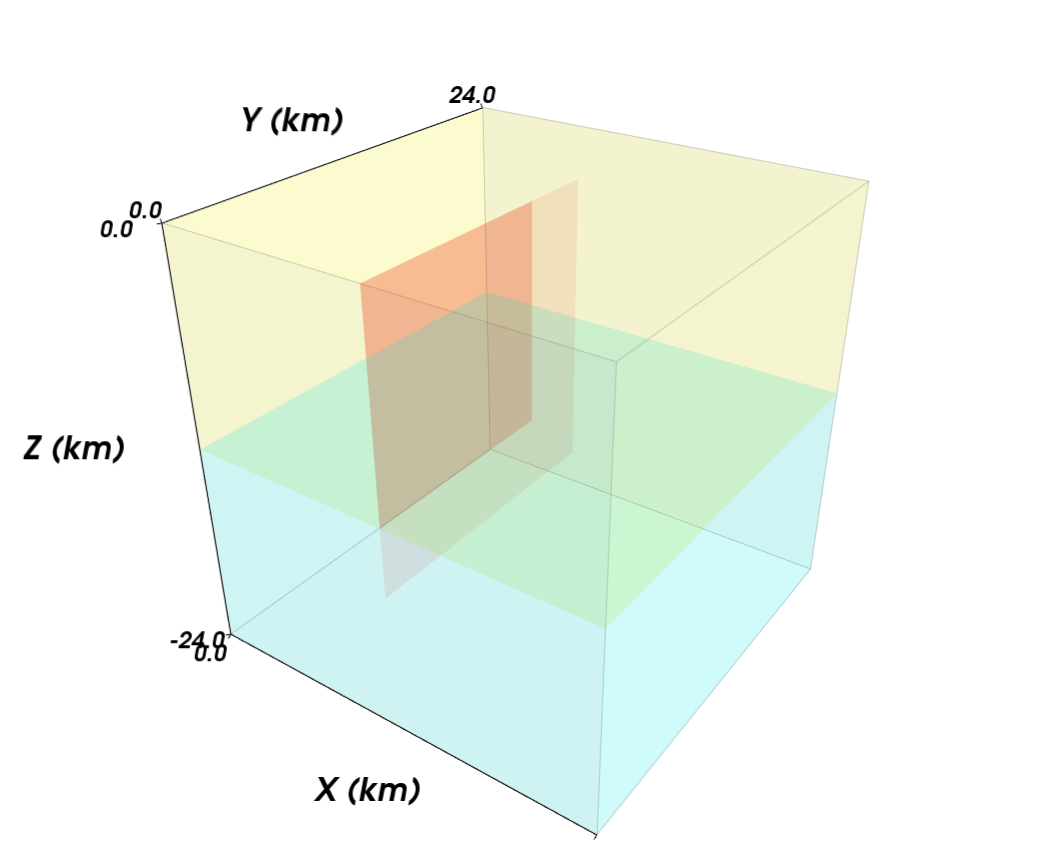
\includegraphics[scale=0.33]{benchmarks/figs/strikeslip_geometry}
   \caption{Geometry of strike-slip benchmark problem.}
   \label{fig:benchmark:strikeslip:geometry}
\end{figure}


\subsection{Running the Benchmark}

Each benchmark uses three {\tt .cfg} files in the parameters
directory: {\tt pylithapp.cfg}, a mesher related file ({\tt
  strikeslip\_cubit.cfg} or {\tt strikeslip\_lagrit.cfg}), and a
resolution and cell related file (e.g., {\tt
  strikeslip\_hex8\_1000m.cfg}).

\begin{shell}
# Checkout the benchmark files from the CIG Git repository.
$ git clone https://github.com/geodynamics/pylith_benchmarks.git
# Change to the quasistatic/sceccrustdeform/strikeslip directory.
$ cd quasistatic/sceccrustdeform/strikeslip
# Decompress the gzipped files in the meshes and parameters
directories.
$ gunzip meshes/*.gz parameters/*.gz
# Change to the parameters directory.
$ cd parameters
# Examples of running static (elastic solution only) cases.
$ pylith strikeslip_cubit.cfg strikeslip_hex8_1000m.cfg
$ pylith strikeslip_cubit.cfg strikeslip_hex8_0500m.cfg
$ pylith strikeslip_cubit.cfg strikeslip_tet4_1000m.cfg
# Append timedep.cfg to run the time-dependent (viscoelastic cases).
$ pylith strikeslip_cubit.cfg strikeslip_hex8_1000m.cfg timedep.cfg
$ pylith strikeslip_cubit.cfg strikeslip_hex8_0500m.cfg timedep.cfg
$ pylith strikeslip_cubit.cfg strikeslip_tet4_1000m.cfg timedep.cfg
\end{shell}

This will run the problem for 10 years, using a time-step size of 0.1
years, and results will be output for each year. The benchmarks at
resolutions of 1000 m, 500 m, and 250 m require approximately 150 MB,
960 MB, and 8 GB, respectively.


\subsection{Benchmark Results}

Figure \vref{fig:benchmark:strikeslip:solution} shows the displacement
field from the simulation with hexahedral cells using trilinear basis
functions at a resolution of 1000 m. For each resolution and set of
basis functions, we measure the accuracy by comparing the numerical
solution against the semi-analytical Okada solution \cite{Okada:1992}.
We also compare the accuracy and runtime across resolutions and different
cell types. This provides practical information about what cell types
and resolutions are required to achieve a given level of accuracy
with the shortest runtime.

\begin{figure}[htbp]
  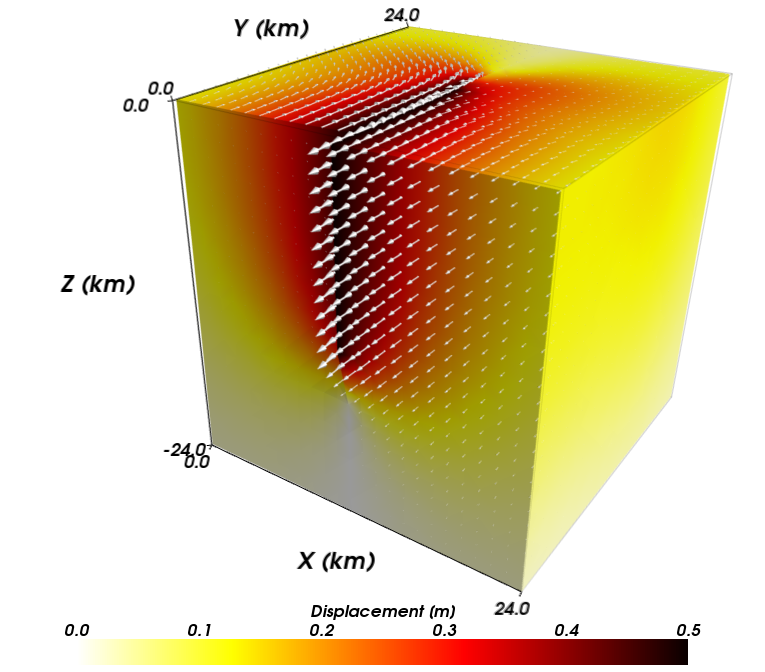
\includegraphics[scale=0.33]{benchmarks/figs/strikeslip_soln}
  \caption{Displacement field for strike-slip benchmark problem.}
  \label{fig:benchmark:strikeslip:solution}
\end{figure}

\subsubsection{Solution Accuracy}

We quantify the error in the finite-element solution by integrating
the L2 norm of the difference between the finite-element solution
 and the semi-analytical solution evaluated at the quadrature points.
We define the local error (error for each finite-element cell) to
be
\begin{equation}
\epsilon_{local}=\frac{1}{V_{cell}}\sqrt{\intop_{cell}\left(u_{i}^{t}-u_{i}^{fem}\right)^{2}\: dV},
\end{equation}
where $u_{i}^{t}$ is the ith component of the displacement field
for the semi-analytical  solution, and $u_{i}^{fem}$ is the ith component
of the displacement field for the finite-element  solution.  Taking
the square root of the L2 norm and normalizing by  the volume of the
cell results in an error metric with dimensions of length.  This roughly
corresponds to the error in the magnitude of the displacement field
in the finite element solution. We define the global error in a similar
fashion,
\begin{equation}
\epsilon_{global}=\frac{1}{V_{domain}}\sqrt{\intop_{domain}\left(u_{i}^{t}-u_{i}^{fem}\right)^{2}\: dV},
\end{equation}
 where we sum the L2 norm computed for the local error over all of
the  cells before taking the square root and dividing by the volume
of the domain. CIG has developed a package called Cigma \url{geodynamics.org/cig/software/packages/cs/cigma}
that computes these local and global error metrics.

Figures \vref{fig:benchmark:strikeslip:tet4:1000m} through \vref{fig:benchmark:strikeslip:hex8:250m}
show the local error for each of the three resolutions and two cell
types. The error decreases with decreasing cell size as expected for
a converging solution. The largest errors, which approach 1 mm for
1 m of slip for a discretization size of 250 m, occur where the gradient
in slip is discontinuous at the boundary between the region of uniform
slip and linear taper in slip. The linear basis functions cannot match
this higher order variation. The trilinear basis functions in the
hexahedral element provide more terms in the polynomial defining the
variation in the displacement field within each cell compared to the
linear basis functions for the tetrahedral cell. Consequently, for
this problem the error for the hexahedral cells at a given resolution
is smaller than that for the tetrahedral cells. Both sets of cell
types and basis functions provide the same rate of convergence as
shown in Figure \vref{fig:benchmark:strikeslip:convergence}.

\begin{figure}[htbp]
  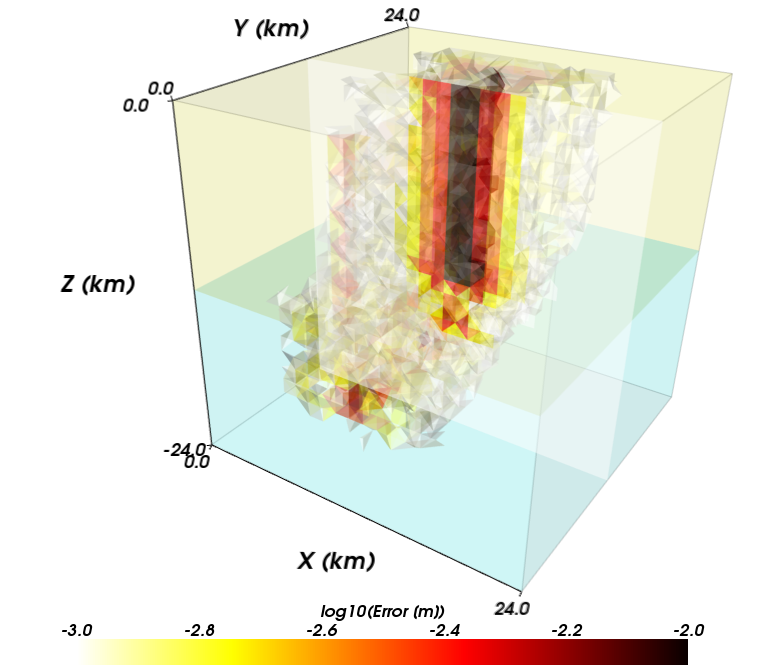
\includegraphics[scale=0.33]{benchmarks/figs/strikeslip_error_tet4_1000m}
  \caption{Local error for strike-slip benchmark problem with
    tetrahedral cells and linear basis functions with a uniform
    discretization size of 1000 m.}
  \label{fig:benchmark:strikeslip:tet4:1000m}
\end{figure}

\begin{figure}[htbp]
  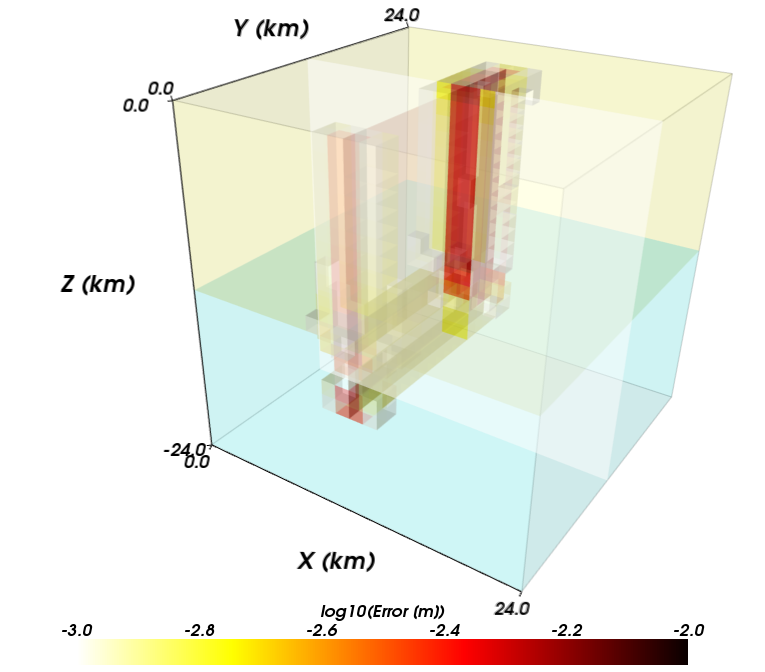
\includegraphics[scale=0.33]{benchmarks/figs/strikeslip_error_hex8_1000m}
  \caption{Local error for strike-slip benchmark problem with
    hexahedral cells and trilinear basis functions with a uniform
    discretization size of 1000 m.}
\label{fig:benchmark:strikeslip:hex8:1000m}
\end{figure}

\begin{figure}[htbp]
  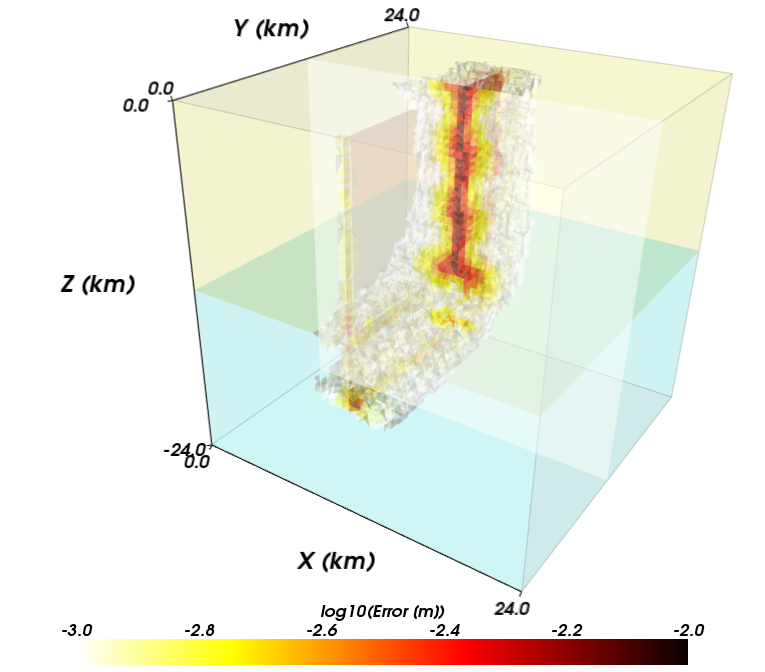
\includegraphics[scale=0.33]{benchmarks/figs/strikeslip_error_tet4_0500m}
  \caption{Local error for strike-slip benchmark problem with
    tetrahedral cells and linear basis functions with a uniform
    discretization size of 500 m.}
\label{fig:benchmark:strikeslip:tet4:500m}
\end{figure}

\begin{figure}[htbp]
  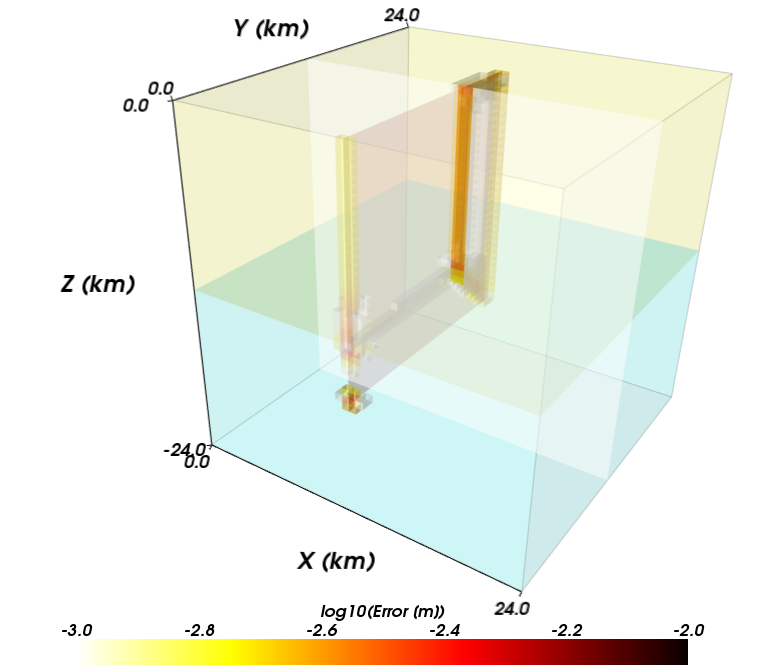
\includegraphics[scale=0.33]{benchmarks/figs/strikeslip_error_hex8_0500m}
  \caption{Local error for strike-slip benchmark problem with
    hexahedral cells and trilinear basis functions with a uniform
    discretization size of 500 m.}
  \label{fig:benchmark:strikeslip:hex8:500m}
\end{figure}

\begin{figure}[htbp]
  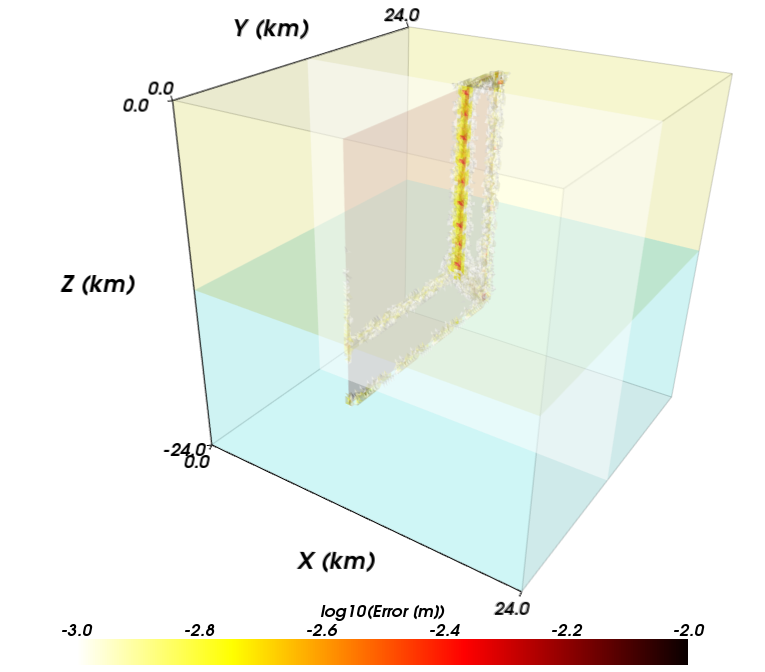
\includegraphics[scale=0.33]{benchmarks/figs/strikeslip_error_tet4_0250m}
  \caption{Local error for strike-slip benchmark problem with
    tetrahedral cells and linear basis functions with a uniform
    discretization size of 250 m.}
  \label{fig:benchmark:strikeslip:tet4:250m}
\end{figure}

\begin{figure}[htbp]
  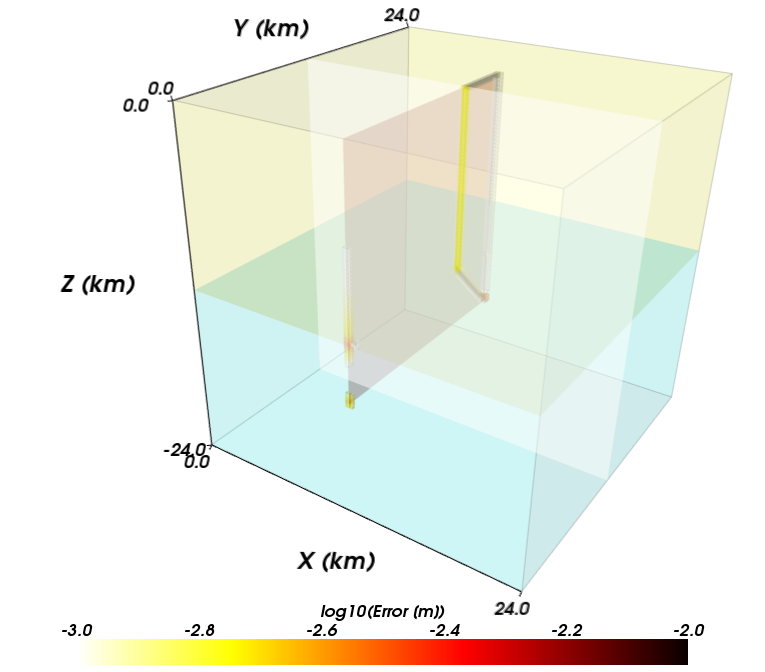
\includegraphics[scale=0.33]{benchmarks/figs/strikeslip_error_hex8_0250m}
  \caption{Local error for strike-slip benchmark problem with
    hexahedral cells and trilinear basis functions with a uniform
    discretization size of 250 m.}
  \label{fig:benchmark:strikeslip:hex8:250m}
\end{figure}

\begin{figure}[htbp]
  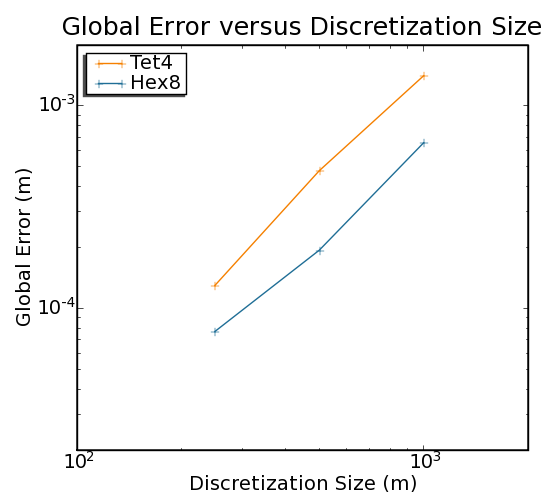
\includegraphics[scale=0.33]{benchmarks/figs/strikeslip_convergence}
  \caption{Convergence rate for the strike-slip benchmark problem with
    tetrahedral cells and linear basis functions and with hexahedral
    cells with trilinear basis functions.}
  \label{fig:benchmark:strikeslip:convergence}
\end{figure}

\subsubsection{Performance}

Figure \vref{fig:benchmark:strikeslip:summary} summarizes the overall
performance of each of the six simulations. Although at a given resolution,
the number of degrees of freedom in the hexahedral and tetrahedral
meshes are the same, the number of cells in the tetrahedral mesh is
about six times greater. However, we use only one integration point
per tetrahedral cell compared to eight for the hexahedral cell. This
leads to approximately the same number of integration points for the
two meshes, but the time required to unpack/pack information for each
cell from the finite-element data structure is greater than the time
required to do the calculation for each quadrature point (which can
take advantage of the very fast, small memory cache in the processor).
As a result, the runtime for the simulations with hexahedral cells
is significantly less than that for the tetrahedral cells at the same
resolution. 

\begin{figure}[htbp]
  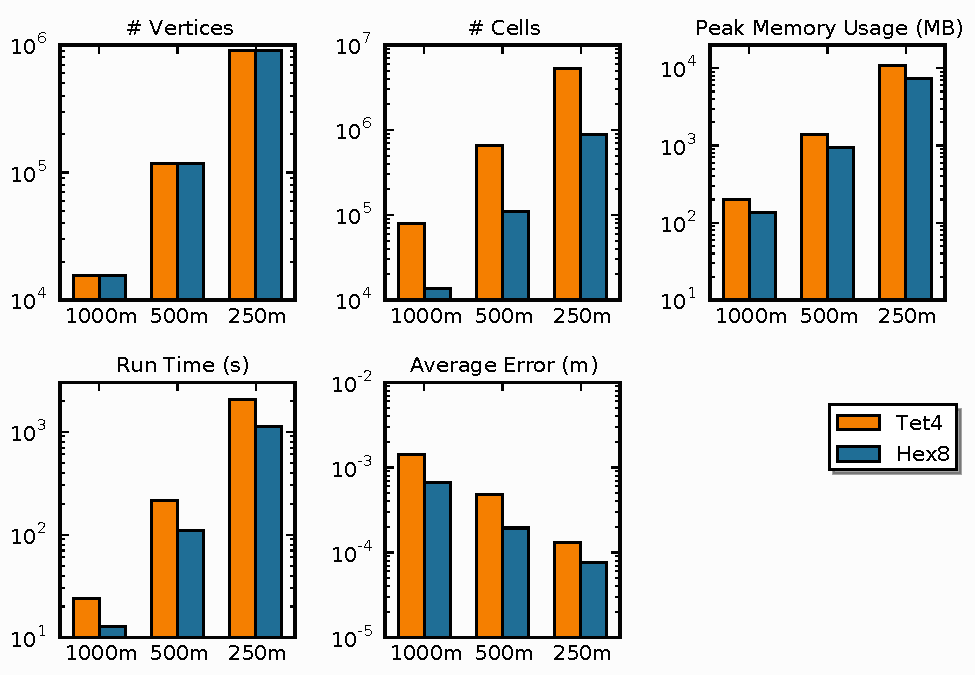
\includegraphics[scale=0.5]{benchmarks/figs/strikeslip_summary}
  \caption{Summary of performance of PyLith for the six simulations of
    the strike-slip benchmark. For a given discretization size,
    hexahedral cells with trilinear basis functions provide greater
    accuracy with a shorter runtime compared with tetrahedral cells
    and linear basis
    functions.}
  \label{fig:benchmark:strikeslip:summary}
\end{figure}

Figure \vref{fig:benchmark:strikeslip:scaling} compares the runtime
for the benchmark (elastic solution only) at 500 m resolution for
1 to 16 processors. The total runtime is the time required for the
entire simulation, including initialization, distributing the mesh
over the processors, solving the problem in parallel, and writing
the output to VTK files. Some initialization steps, writing the output
to VTK files, and distributing the mesh are essentially serial processes.
For simulations with many time steps these steps will generally occupy
only a fraction of the runtime, and the runtime will be dominated
by the solution of the equations. Figure \vref{fig:benchmark:strikeslip:scaling}
also shows the total time required to form the Jacobian of the system,
form the residual, and solve the system. These steps provide a more
accurate representation of the parallel-performance of the computational
portion of the code and show excellent performance as evident in the
approximately linear slope of 0.7. S linear decrease with a slope
of 1 would indicate strong scaling, which is rarely achieved in real
applications.

\begin{figure}[htbp]
  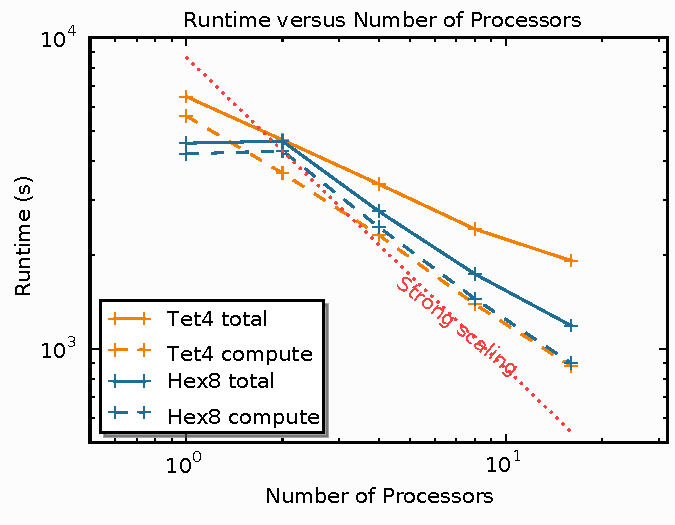
\includegraphics[scale=0.75]{benchmarks/figs/strikeslip_scaling}
  \caption{Parallel performance of PyLith for the strike-slip
    benchmark problem with tetrahedral cells and linear basis
    functions with a uniform discretization size of 500 m. The total
    runtime (total) and the runtime to compute the Jacobian and
    residual and solve the system (compute) are shown.  The compute
    runtime decreases with a slope of about 0.7; a linear decrease
    with a slope of 1 would indicate strong scaling, which is rarely
    achieved in any real
    application.}
  \label{fig:benchmark:strikeslip:scaling}
\end{figure}

% End of file
